\documentclass[12pt,fleqn]{article}\usepackage{../../common}
\begin{document}
Logaritmayı Taylor Serisi İle Hesaplamak

Taylor açılımı tekniğini ilk gördüğümüzde öğrenci genelde kendine şu soruyu
sorar: "İyi ama, bu ne işe yarar?" Taylor serilerini ilginç kılan özellik,
bir formülü bir başkasına dönüştürmemizi sağlamaları, ve, genelde sonsuz
olmayan bir formülü, sonsuza kadar devam eden terimlerin toplamı olan başka
bir formül ile değiştirmemizi sağlamalarıdır.

Sonsuza kadar devam eden terimler toplamı, karışık bir durumdur. Teklikten,
çokluğa niye gidilmektedir? Bu sonsuz terimler dizisi ne işe yaramaktadır?
Öğrenciye göre, düzenden, düzensizliğe gidilmiştir. Niçin? Bu tür sorular,
Taylor serilerinin tanıştırıldığı her derste cevaplanmalıdır. Bu yazıda,
Taylor serisinin ne işe yaradığını, hangi problemler için kullanıldığını,
ve ait olduğu matematiksel dünyanın hangisi olduğunu göreceğiz.

Yaklaşıklamak (Approximation)

Yaklaşıklamak, bir değeri, fonksiyonu, matematiksel bir kavramın yerine ona
yakın, aşağı yukarı eşit olan başka bir değeri/fonksiyonu/kavramı koymak
demektir. Gündelik hayatta bazı sayıları sürekli başkaları ile
yaklaşıklamaya uğraşmaktayız. Mesela bir alan, uzunluk, hacim, vs. gibi
şeyler ölçerken, mecburen yaklaşıksal kavramlar ile yüzyüze
gelmekteyiz. Normalde gündelik hayatımızda sadece tamsayılar ve
tamsayıların bölümü olarak gösterilebilecek rasyonel sayılar kullanırız,
fakat matematikte rasyonel sayıların yanında, irrasyonel sayılar da
mevcuttur. Ölçümlerimiz sırasında irrasyonel sayılar ortaya çıkmasalar da,
teorik argümanlarımız ve işlemlerimiz çoğunlukla bizi o yöne doğru
itiverir. Yarıçapı 1/2 olan bir çemberin uzunluğu pi denilen 'irrasyonel'
sayıdır, ya da iki kenarı eşit, bir birim uzunluğunda olan dik üçgenin
hipotenüsü 2'nin kareköküdür, bu sayı da irrasyonel bir
sayıdır. "İrrasyonel" kelimesinin İngilizce'de 'deli', 'üşütük', veya
'mantıksız' olarak karşılık bulması da ilginçtir. İrrasyonel sayılar
virgülden sonra bile sonsuza kadar devam etmektedirler [3].

Bu sebeple, irrasyonel sayılar ile işlem yaparken, onları 'rasyonel' bir
sayı ile yaklaşıklamak gerekir. Bunu yapmak için çoğu zaman virgülden sonra
belli bir basamak sonrasını atarız [3].

Başka bir alanı ele alalım: Doğa bilimleri sürekli fonksiyonlar ile bir
yaklaşıklama eylemi içindedirler. Doğanın ölçümsel gizemleri matematikte
bir fonksiyon olarak gösterilir, ve bu fonksiyonlar hiçbir zaman kesinkes,
tıpatıp her seviyede ve her molekülü anlatan betimler değildir. Elde olan,
yaklaşıksal olarak ve şartlara göre kesinlik derecesi bazen çok, bazen daha
fazla olan bir ibaredir [3].

Bâzen de, doğal şartlara hiç alâkası olmayan "pür matematiksel" bir
fonksiyonu başka bir fonksiyon ile değiştirmeye mecbur kalabiliriz. Bunu
da, genelde başlangıç fonksiyonunu hesaplayabilmek için yaparız [3].

Şimdi yaklaşıklamak istediğimiz log() fonksiyonuna gelelim.

Log Nedir?

$Log(x)$ fonksiyonu en basit şekilde $f(t)=1/t$ fonksiyonunun, 1 değeri ile x
değeri arasında kalan alanıdır [4]. Yani, bu fonksiyonunun entegralinin 1 ile
x değeri arasındaki değeridir (entegralin alan hesapladığını lise
matematiğinden biliyoruz).

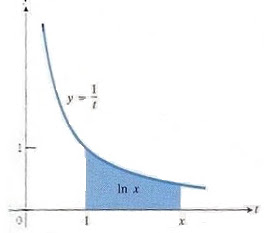
\includegraphics[height=7cm]{taylor_log_graph.jpg}

$$ \ln x = \int _{1}^{x} \frac{1}{t}, \qquad \frac{d(\ln x)}{dx} = \frac{1}{x}$$

Sembolik olarak logaritma fonksiyonu, çarpma işlemlerini toplamaya
çevirmemizi sağladığı için matematiksel olarak çok yararlı bir
araçtır. Zaten, keşfedilme sebebi de budur. Bu yaygın kullanım, uygulamalar
için logaritmanın bir aşamada hesaplanmasını gerektirmektedir. Fakat,
görüldüğü gibi 1/t fonksiyonu entegral işleminden sonra güzel bir
matematiksel fonksiyona dönüşmediği için, yaklaşıksal yöntemlere gereksinim
duymaktayız. Taylor açılımı işte burada imdadımıza yetişmektedir.

Örnek olarak, log(20) işleminin sonucunu Taylor serisinin yardımı ile
hesaplayacağız. Niye Taylor açılımı? Çünkü log fonksiyonunun her dereceden
türevi mevcut, Taylor açılımı için de bu türevler lazım.

Log'un Açılımı

Log fonksiyonunu nasıl açarken, amatör bir başlangıç şöyle
olabilirdi. Dikkat edelim, şu anda sadece sembolik olarak işlem yapıyoruz.

$$ f(x) = \log(x) $$

$$ f'(x) = \frac{1}{x}, f''(x) = \frac{-1}{x^2}, f'''(x)=.. $$

$$ f(x) \approx f(a) + f'(a)(x-a)+\frac{f''(a)}{2!}(x-a)^2 + ... $$

$$ f(x) \approx \log(a) + \frac{1}{a}(x-a) + \frac{\frac{-1}{a^2}}{2!}(x-a)^2 $$

Bu pek derli toplu bir açılım olarak gözükmüyor. $a=0$ seçersek, 

$$ f(x) \approx \log(a) + \frac{1}{a}(x-a) + \frac{\frac{-1}{a^2}}{2!}(x-a)^2 + ..$$

$$ f(x) \approx \log(0) + \frac{1}{a}x + \frac{\frac{-1}{0^2}}{2!}(x)^2 + ..$$

çıkar. $log(0)$ tanımsızdır. Yani bu açılım işimize yaramayacak. Daha temiz
bir açılım için matematikçiler şu yöntemi bulmuştur.

$log(x)$ yerine, $log(1+x)$ kullanalım. 

$$ f(x) = \log(1+x) $$

$$ f'(x) = \frac{1}{1+x}, f''(x) = \frac{-1}{1+x}^2, f'''(x) = ... $$

$$ f(x) \approx f(a) + f'(a)(x-a) + \frac{f'''(a)}{2!}(x-a)^2 + ... $$

$a = 0$ alırsak

$$ f(x) \approx \log(1+a) + \frac{1}{1+a} (x-a)+ \frac{\frac{-1}{(1+a)^2}}{2!} (x-a)^2$$

$$ f(x) \approx \log(1) + \frac{1}{1}(x) + \frac{\frac{-1}{1^2}}{2!} (x)^2$$

$$ f(x) \approx 0 + \frac{1}{1}(x) \frac{\frac{-1}{1^2}}{2!} (x)^2 $$

$$ f(x) \approx x - \frac{x^2}{2!}  + \frac{x^3}{3!} ... $$

Bu çok daha temiz oldu. Dikkat ederseniz, entegrali düzgün olmayan $log()$
fonksiyonunun Taylor açımı ne kadar temiz oldu. Bu fonksiyonu bilgisayar
ile hesaplamak çok basittir. Artık log(20)'yi hesaplamaya hazırız.

$$ f(x) \approx x - \frac{x^2}{2!}  + \frac{x^3}{3!} ... $$

$$ \log(20) \approx 20 - \frac{20^2}{2!} + \frac{20^3}{3!} ... $$

Ama dikkat! Açılan fonksiyonunu hesaplarken x'e verdiğimiz değerin a
noktasına yakın olması önemlidir.

Çok uzak noktalar (yukarıdaki log(20)'nin açılımının olduğu gibi)
elimizdeki yeni seriyi uzaklastiran (diverging) bir seri haline
getirebilir. Bunun tersi olan yakınlasan (converging) seriler, elinizdeki
terim sayısını biz arttırdıkça, sabit bir sayıya doğru yönelen serilere
denir. Bizim amacımız hesap yapmak olduğuna göre, bir somut sayıya doğru
yönelen bir seriyi tabii ki tercih ederiz. Bu sebeple elimizdeki serinin,
istediğimiz x değeri için yakinlasan bir seri mi, yoksa uzaklasan bir seri
mi olduğunu çok iyi bilmek zorundayız.

$log(1+x)$'in Taylor açılımı sadece $-1$ 

Burada, log aritmetiği yardımımıza erişiyor. Log işlemlerinde, bölmenin
çıkarmaya, çarpmanın toplamaya dönüştüğünü hatırlayalım. Yâni Log(x*y) =
log(x) + log(y), ve log(x/y) = log(x) - log(y) olur.

O zaman, $\log(20)$'yi 1'den küçük sayılar kullanacak şekilde yeniden
yazalım:

$$ 
\log(20) = \log( \frac{\frac{1}{2}}{\frac{1}{40}}) = \log(\frac{1}{2})-\log(\frac{1}{40})
$$

$$ \log(1+x) \approx x - \frac{x^2}{2!} + \frac{x^3}{3!} $$

Not: $(1+x)$'in $\frac{1}{2}$ vermesi için $x$'in $-\frac{1}{2}$ olması
gerekir. 

$$ 
log(\frac{1}{2}) \approx -\frac{1}{2} - \frac{-\frac{1^2}{2}}{2!}  + 
\frac{-\frac{1^3}{2}}{3!} - ...
$$

Aynı şekilde $1/40$ için durum aynıdır.

$$ 
log(\frac{1}{40}) \approx
-\frac{39}{40} -
\frac{-\frac{39^2}{40}}{2!} -
\frac{-\frac{39^3}{40}}{3!} + ...
$$

Bu kadar! Sağ tarafta gözüken serilerin hesabını, bir Python programı 
ile yaptık.

\begin{minted}[fontsize=\footnotesize]{python}

def taylor_ile_log(bolum, bolen, taylor_ile_acilim_buyuklugu):
    sum = 0
    for i in range(1,taylor_ile_acilim_buyuklugu):
        sum += np.power(-1, i+1) * (np.power(bolum/bolen, i) / i)

    return sum
        
print taylor_ile_log(-39.0, 40.0, 160)
\end{minted}

\begin{verbatim}
-3.68527101165
\end{verbatim}
LISP

\begin{minted}[fontsize=\footnotesize]{common-lisp}
;;
;; Not: (/ 1 2) yazilirsa, Common Lisp 0 cevabi veriyor.
;; Bunun sebebi, 1 2 deyince, parametrelerin integer 
;; (tamsayi) olarak anlasilmasiymis, parametreler tamsayi 
;; olunca, sonucta tamsayi olarak donuyor. O yuzden kesirli 
;; cevaplar almak icin, (/ 1.0 2.0) demek lazim. 

;;;;;;;;;;;;;;;;;;;;;;;;;;;;;;;;;;;;;;;;;;;;;;;;;;;;;;

(defun power (Base Exponent)
  "Reproduced EXPT in case where Exponent is non-negative integer"
  (cond
    ((= Exponent 0)  1)
    ((evenp Exponent)(Power (* Base Base) (/ Exponent 2))) 
    (t               (* Base (Power Base (- Exponent 1))))) )

;;;;;;;;;;;;;;;;;;;;;;;;;;;;;;;;;;;;;;;;;;;;;;;;;;;;;;

(defun basit-taylor-ile-log-of-1-bolu-2 ()
   (+ 
    (* +1 ;;; taylor serisinin birinci terimi
       (/
	(power (/ -1.0 2.0)
	       1)
	1)
       )
    (* -1 ;;; taylor serisinin ikinci terimi
       (/
	(power (/ -1.0 2.0)
	       2)
	2)
       )
    (* +1 ;;; taylor serisinin ucuncu terimi
       (/
	(power (/ -1.0 2.0)
	       3)
	3)
       )
    ;
    ; vs...vs..
    ;
    )
  )

;;;;;;;;;;;;;;;;;;;;;;;;;;;;;;;;;;;;;;;;;;;;;;;;;;;;;;
(defun taylor-ile-log-hesapla (bolum bolen taylor-acilim-buyuklugu)
  (let ((sum 0)(i 1))
    (loop for i from 1 to taylor-acilim-buyuklugu do
	  (setq sum (+ sum (* (power -1 (+ i 1))
			      (/
			       (power (/ bolum bolen)
				      i)
			       i)
			      )))
	  )
    sum)
)


(print "------------- 1/2 (yani log( 1 + (-1/2)) Hesabi -----")
(print "Basit kod")
(print (basit-taylor-ile-log-of-1-bolu-2))
(print "Daha cok taylor terimi kullanan kod")
(print (taylor-ile-log-hesapla -1.0 2.0 100))
(print "Bilgisayarin kendi log()'undan gelen sonuc")
(print (log (/ 1.0 2.0)))

(print "------------- 1/40 (yani log( 1 + (-39/40)) ------- ")
(print "160 taylor terimi")
(print (taylor-ile-log-hesapla -39.0 40.0 160))
(print "180 taylor terimi")
(print (taylor-ile-log-hesapla -39.0 40.0 180))
(print "200 taylor terimi")
(print (taylor-ile-log-hesapla -39.0 40.0 200))
(print "220 taylor terimi")
(print (taylor-ile-log-hesapla -39.0 40.0 220))
(print "240 taylor terimi")
(print (taylor-ile-log-hesapla -39.0 40.0 240))
(print "260 taylor terimi")
(print (taylor-ile-log-hesapla -39.0 40.0 260))
(print "Bilgisayarin kendi algoritmasina gore log(1/40)")
(print (log (/ 1.0 40.0)))
(print "--------------- Sonuc --------------------- ")

(print "log(1/2) - log(1/40)")
(print (- (taylor-ile-log-hesapla -1.0 2.0 100)
	  (taylor-ile-log-hesapla -39.0 40.0 200)))

(print "Bilgisayarin mevcut algoritmasinin verdigi ")
(print (log 20))
\end{minted}

Kaynaklar

[3] Thomas, {\em Thomas' Calculus}

\end{document}
